\documentclass[tikz,border=2pt]{standalone}
\usepackage{amsmath,amssymb}
\usepackage{tikz}
\usetikzlibrary{arrows.meta}

\begin{document}
% A spanning list reaches every vector of the space, but it may be redundant: with three
% vectors in the plane the same w has several representations.
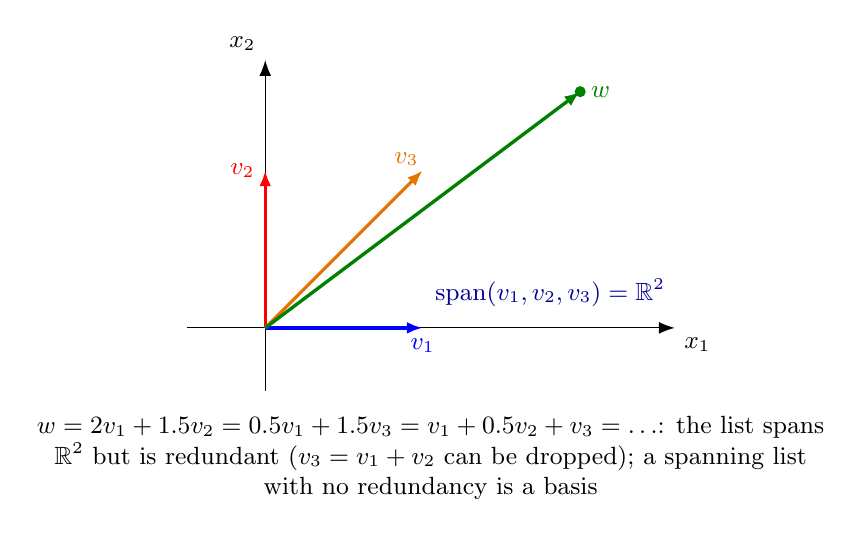
\begin{tikzpicture}[every node/.style={font=\small}, >={Latex[length=2mm]}]
	\draw[->] (-1,0) -- (5.2,0) node[below right] {$x_1$};
	\draw[->] (0,-0.8) -- (0,3.4) node[above left] {$x_2$};
	\draw[->, blue, very thick] (0,0) -- (2,0) node[below] {$v_1$};
	\draw[->, red, very thick] (0,0) -- (0,2) node[left] {$v_2$};
	\draw[->, orange!90!black, very thick] (0,0) -- (2,2) node[above left, inner sep=1pt] {$v_3$};
	\draw[->, green!50!black, very thick] (0,0) -- (4,3) node[right] {$w$};
	\fill[green!50!black] (4,3) circle (2pt);
	\node[blue!60!black, anchor=south east] at (5.2,0.15) {$\operatorname{span}(v_1,v_2,v_3)=\mathbb{R}^2$};
	\node[anchor=north, align=flush center, text width=10cm] at (2.1,-1.0) {$w=2v_1+1.5v_2=0.5v_1+1.5v_3=v_1+0.5v_2+v_3=\ldots$: the list spans $\mathbb{R}^2$ but is redundant ($v_3=v_1+v_2$ can be dropped); a spanning list with no redundancy is a basis};
\end{tikzpicture}
\end{document}
